\documentclass[11pt,a4paper,twoside]{report}
\usepackage{hyperref}
\usepackage{graphicx}
\usepackage{soul}
\usepackage{algorithm}
\usepackage[noend]{algorithmic}

\newcommand{\Csharp}{%
  {\settoheight{\dimen0}{C}C\kern-.05em \resizebox{!}{\dimen0}{\raisebox{\depth}{\#}}}}

\begin{document}

\tableofcontents

\chapter{How to join the BigARTM project?}
\begin{enumerate}
\item Source code is hosted in a private github repository.
    If you don't have a user on github, please register a free user \href{https://github.com/}{here}.
    Then send the name of your github user to \href{mailto:sashafrey@gmail.com}{sashafrey@gmail.com},
    using ``BigARTM: request access'' in the title of your e-mail.
    In few days you will receive a reply confirming that access had been granted.
\item To clone the repository and build sources, please refer to paragraph
    \hyperref[label:how_to_build]{How to build sources}.
\item Read about the math behind BigARTM library: \\ \url{http://www.machinelearning.ru/wiki/images/2/22/Voron-2013-ptm.pdf}
\item Review the list of open issues: \\
    \url{https://github.com/sashafrey/topicmod/issues?state=open}\\
    Feel free to select some of them which sounds interesting and assign it to yourself.
    To submit you change, follow \hyperref[label:how_to_submit]{How to submit my change} guide.
\item Review the latest discussions here: \\
    \url{https://groups.google.com/forum/#!forum/artm_dev}
\end{enumerate}

\chapter{BigARTM - internal documentation}

\section{Intro}
ToDo: write short gentle introduction that provide links to state of the art articles on topic models and BigARTM.

\paragraph{Main goals for the first release.}
\begin{itemize}
    \item Implementation of core topic modeling algorithms with ARTM (Additive Regularization of Topic Models)
    \item Prefer online algorithms, that do not require storing complete doc-token matrix in memory
    \item Utilize sparsity of doc-token and token-topic matrices
    \item Scale well for 32 CPU cores and higher, efficiently using shared memory within single process
    \item Exhibit high convergence rates
    \item Be portable (written in C/C++, tested with gcc, intel and cl.exe)
    \item Have an interface in Python, Java and $\Csharp$
    \item Be open-source (MIT license)
\end{itemize}
First version we release to public may not have the following features:
\begin{itemize}
    \item Distributed cluster solution
    \item CUDA and Intel Xeon Phi support
\end{itemize}
This is likely to be added in later versions.

\paragraph{Success criteria.}
When codebase meets this success criteria we are free to release the library.
\begin{itemize}
    \item The algorithm scales linearly up to 32 CPU cores when process
    \href{http://archive.ics.uci.edu/ml/datasets/Bag+of+Words}{pubmed task}.
    \item On small datasets perplexity of our method is on parity with other libraries
    \item Builds with gcc, intel and cl.exe compiler; runs on Ubuntu, Solaris and Windows.
    \item No crashes, hangs or memory leaks in stress testing against real-world and model datasets
    \item Convergence rate is well understood
    \item Performance model is well understood (Disk, Memory, CPU)
\end{itemize}

\section{Design}

\subsection{Online Batch PLSA algorithm}

Design of the BigARTM library is driven by Online Batch PLSA algorithm,
(Fig. \ref{fig:plsa_alg}).

\begin{algorithm}
\caption{Online Batch PLSA algorithm}
\label{fig:plsa_alg}
\begin{algorithmic}[1]
\STATE Initialize $\phi^0_{wt}$ for all $w \in W$ and $t \in T$;
\FORALL{$i = 1, \dots, I$}
    \STATE $n^i_{wt} := 0, n^i_t := 0$ for all $w \in W$ and $t \in T$;
    \FORALL{batches $D_j$, j = 1,...,J}
		\STATE $\tilde n_{wt} := 0, \tilde n_t := 0$ for all $w \in W$ and $t \in T$;
		\FORALL{ $d \in D_j$}
			\STATE initialize $\theta_{td}$ for all $t \in T$;
			\REPEAT
				\STATE $Z_w := \sum_{t \in T} \phi^{i-1}_{wt} \theta_{td}$ for all $w \in d$;
				\STATE $\theta_{td} := \frac{1}{n_d} \sum_{w \in d} n_{dw} \phi^{i-1}_{wt} \theta_{td} / Z_w$
                       for all $t \in T$;
			\UNTIL{$\theta_d$ converges};
			\STATE increment $\tilde n_{wt}, \tilde n_t$ by $n_{dw} \phi^{i-1}_{wt} \theta_{td} / Z_w$
                   for all $w \in W$ and $t \in T$;
		\ENDFOR
        \STATE $n^i_{wt} := n^i_{wt} + \tilde n^i_{wt}$ for all $w \in W$ and $t \in T$;
        \STATE $n^i_t := n^i_t + \tilde n_t$ for all $t \in T$;
    \ENDFOR
	\STATE $\phi^{i}_{wt} := \frac{n^i_{wt}}{n^i_{t}}$
           for all $w \in W$ and $t \in T$;
\ENDFOR
\end{algorithmic}
\end{algorithm}

In this algorithm most CPU resources are consumed on steps $8$~--~$11$
to infer the $\theta_{td}$ distribution for each document.
This operation can be executed concurrently across documents or batches.
In BigARTM this parallelization is done across batches to avoid splitting the work into too small junks.

Processing each batch produces counters $\tilde n_{wt}$ and $\tilde n_{t}$,
which should be then merged with the corresponding counters coming from other batches.
Since this information is produced by multiple concurrent threads
the merging process should be thread-safe and properly synchronised.
Our solution is to store all counters $\tilde n_{wt}$ and $\tilde n_{t}$ into a single queue,
from where they can be picked up by a single \emph{merger thread}.
This thread will then accumulate the counters without any locking.

Further in this text the term \emph {outer iteration loop} stands for the loop at the step $2$,
and the term \emph{inner iteration loop} stands for the loop at step $8$.
Instead of 'repeat until it converges' criteria
current implementation uses a fixed number of iterations,
which is configured manually by the user.

Step $15$ is incorporated into all steps that require $\phi_{wt}$
(e.g. into steps $9$, $10$ and $11$).
These steps utilize counters from the previous iteration ($n^{i-1}_wt$ and $n^{i-1}_t$),
which are no longer updated by the merger thread, hence they represent read-only data
and can be accessed from multiple threads without any synchronization.
At the same time the merger thread will accumulate counters for $n^i_{wt}$ and $n^i_t$
for the current iteration, again in a lock-free manner.

\subsection{User API}
This chapter describes BigARTM from the user perspective, before diving into all implementation details in the next chapters.

From the user perspective BigARTM library can be used either in \emph{local mode} or in \emph{network mode}.
In local mode the user interacts with the library only through the \emph{Master component}.
Typical usage of Master component involves the following steps:
\begin{enumerate}
\item Specify general parameters in \emph{MasterComponentConfig}
\item Create definitions of topic models and their regularizers
\item Load collection of documents to use in topic modeling
\item Invoke iterative scans over the collection and wait until it is competed
\item Retrieve results, including topic model, scores such as perplexity, etc.
\end{enumerate}

In network mode user interacts with the Master component in exactly the same way
as in local mode.
That only action to be done at remote machines is to launch
there a \emph{Node controller} component
and configure it with the endpoint of the Master component.
Then master component will connect to the remote nodes and use them for calculation.
Further details on network mode are provided in section \ref{label:network_modus_operandi}.

\subsection{BigARTM internal architecture}

The key internal components of BigARTM are \emph{DataLoader}, \emph{Processor}, and \emph{Merger}.
Interaction between these components is orchestrated by a class called \emph{Instance},
and two queues --- the \emph{processors queue}, and the \emph{merger queue}.
All functionality is wrapped and exposed to user via \emph{MasterComponent} and \emph{NodeController}.

Please, refer to Fig. \ref{fig:diagramm_artm_core} and \ref{fig:diagramm_workflow}
for the overall architecture diagram and typical user workflow.

\begin{figure}[h!]
\begin{centering}
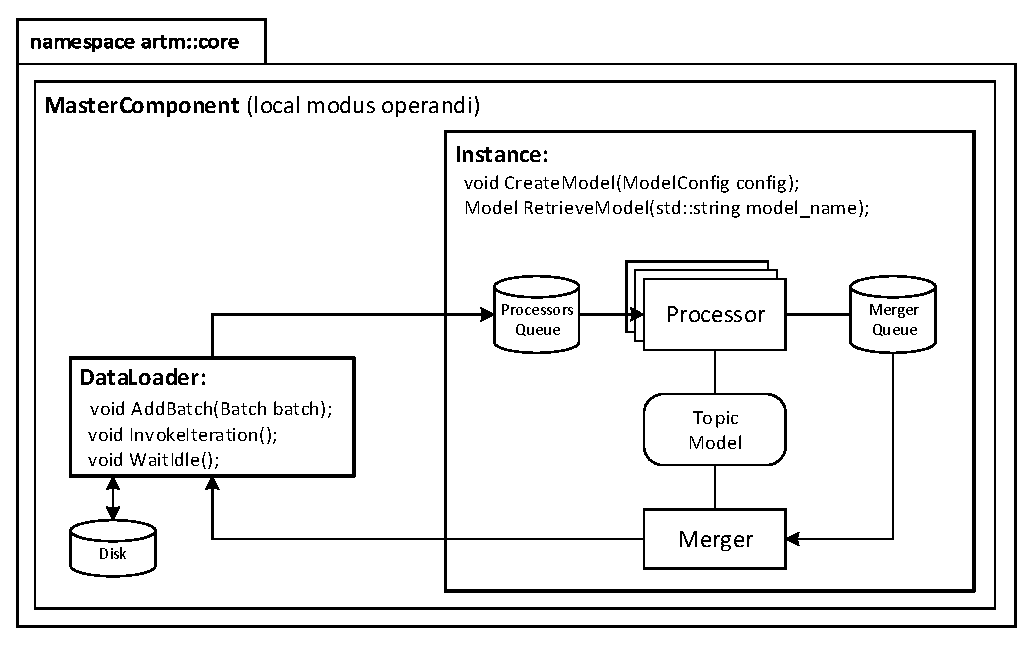
\includegraphics[height=64mm]{diagramm_artm_core.eps}
\caption{Diagram of core ARTM components}
\label{fig:diagramm_artm_core}
\end{centering}
\end{figure}
\vspace{1ex}

\begin{figure}[h!]
\begin{centering}
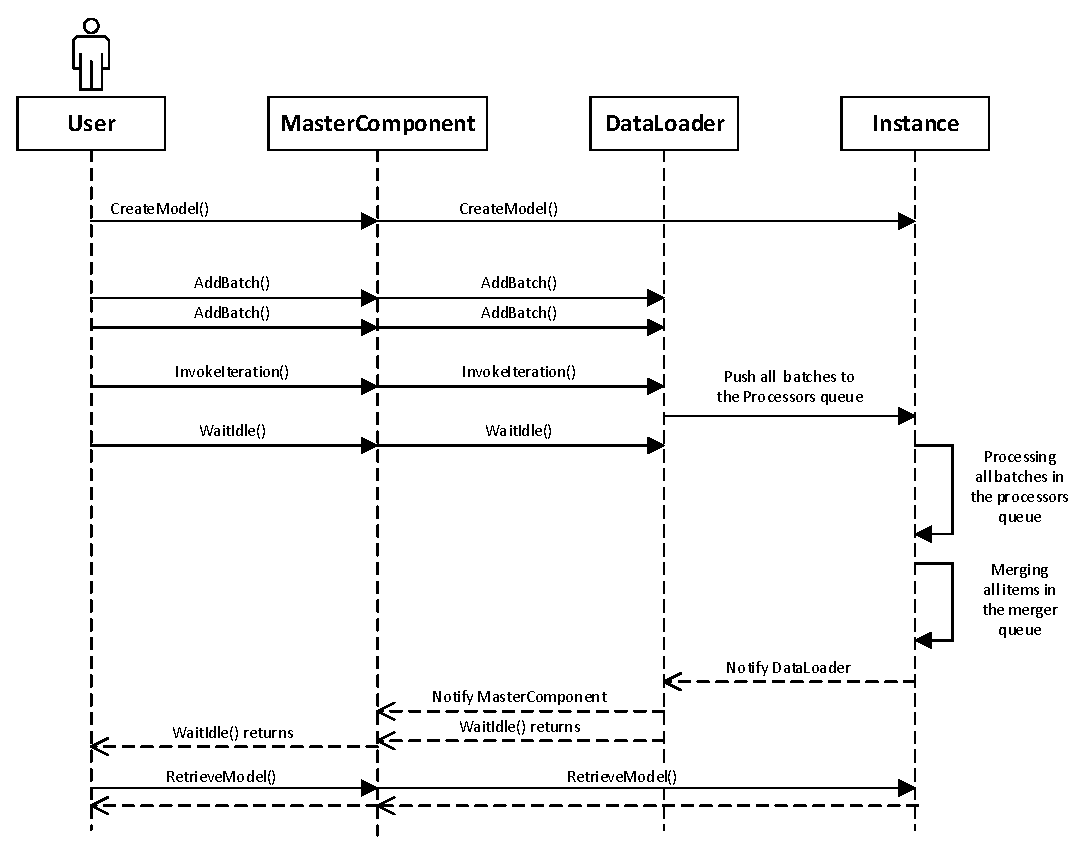
\includegraphics[width=90mm]{diagramm_workflow.eps}
\caption{Interaction between User and BigARTM components}
\label{fig:diagramm_workflow}
\end{centering}
\end{figure}

\textbf{DataLoader.} Responsibility of DataLoader component is to populate the the processors queue
with batches of data (small chunks of the collection).
It is up to implementation of the DataLoader to decide where to gather batches
(they can be stored in memory, on disk, or even came through the network).
DataLoader can be told to trigger a scan over the whole collection,
and then wait for the scan to be finished.

It is possible to set up several \emph{streams} inside DataLoader
(for example, one stream for training items, and the other for test items).
Models (and quality measures such as perplexity) specify which stream to use for tuning (evaluation).

\textbf{Processor.} Processor component withdraws batches from the processors queue
and infers a distribution of the documents into topics.
The output is stored in \emph{merger queue}.
Before processing a new batch the processor asks merger about the the latest token-topic matrix.

If processor observes a token that is not part of token-token matrix, it stores this token in the list of
new ``discovered'' tokens, and transfers this list as part of processor output.
Merger picks up all such tokens, and initializes new row in token-topic matrix.
So, during the first scan over the collection the dictionary is gathered automatically.

\textbf{Merger.}
Merger reads the merger queue and updates token-topic matrix.
At any moment there exist two copies of token-topic matrix,
an ``active'' and a ``background''.
The ``active'' token-topic matrix is used by processors,
while ``background'' token-topic matrix can be safely updated by merger.
At the end of each outer iteration merger will switch the ``active''
token-topic matrix to latest ``background'' matrix,
and start collecting the background matrix from scratch.
Even after switching ``active'' topic-matrix the previous (deprecated) active matrix
will be in use to complete all ongoing processing of batches.
Every new batch will be processed with a new matrix.

This design should be able to utilize CUDA-enabled devices or Index Xeon Phi co-processor
by implementing a special processor, without any changes in the rest of the architecture.
For CUDA the most promising parallelization is to assign CUDA-threads to topic
while inferring a doc-topic distribution.
DataLoader implements caching, so that if the whole collection fits into memory
it does not have to reload index parts from disk for the second and further scans.

\subsection{Network modus operandi}
\label{label:network_modus_operandi}

In network modus operandi master component no longer hosts any processors,
and all computation is therefore transferred to the remote nodes.
Master component became responsible for the following operations:
\begin{enumerate}
\item Keeping track of all remote nodes
\item Reconfiguring all remote nodes once the user reconfigures the master component
      (including updates of ModelConfig and RegularizerConfig)
\item Hosting the latest token-topic matrix, and updating it with increments produced on remote nodes
\item Distribution of the latest token-topic matrix to the remote nodes
\item Calculation of Phi-regularizers
\item During the outer iteration to dynamically distribute the batches across the remote nodes
\end{enumerate}

Fig. \ref{fig:diagramm_artm_network} represents the architecture diagram of BigARTM in network modus operandi.
Compare it with Fig. \ref{fig:diagramm_artm_core}, which represents the local modus operandi.
Note that the key  ``DataLoader $\rightarrow$ Processor $\rightarrow$ Merger'' workflow
at the nodes is similar to the workflow of the MasterComponent in local modus operandi.
Few important things to remember:
\begin{itemize}
    \item In network mode master component has to be configured with a network endpoint,
          accessible by all node controllers
    \item Master component has to be configured with the disk path location which refers
          to a network file share, accessible by all nodes
    \item Currently the master component shell be launched earlier than all other nodes.
          It is the node controller who initializes the connection with the master component.
          \emph{ToDo: we should fix this so that MasterComponent can connect to all nodes in a predefined list}
    \item Currently the master component does not reconfigure automatically reconfigure newly connected nodes.
          A new Reconfigure() operation should be issued on MasterComponent
          after all nodes are connected in order to push the configuration to the nodes.
    \item Some important operations, such as regularization of Phi matrix,
          are not yet implemented in the network modus operandi.
    \item Error handling is not yet implemented in network modus operandi,
          so it is expected to get crashes or undefined behaviour due to minor network glitches.
          This will be fixed.
\end{itemize}

\begin{figure}[h!]
\begin{centering}
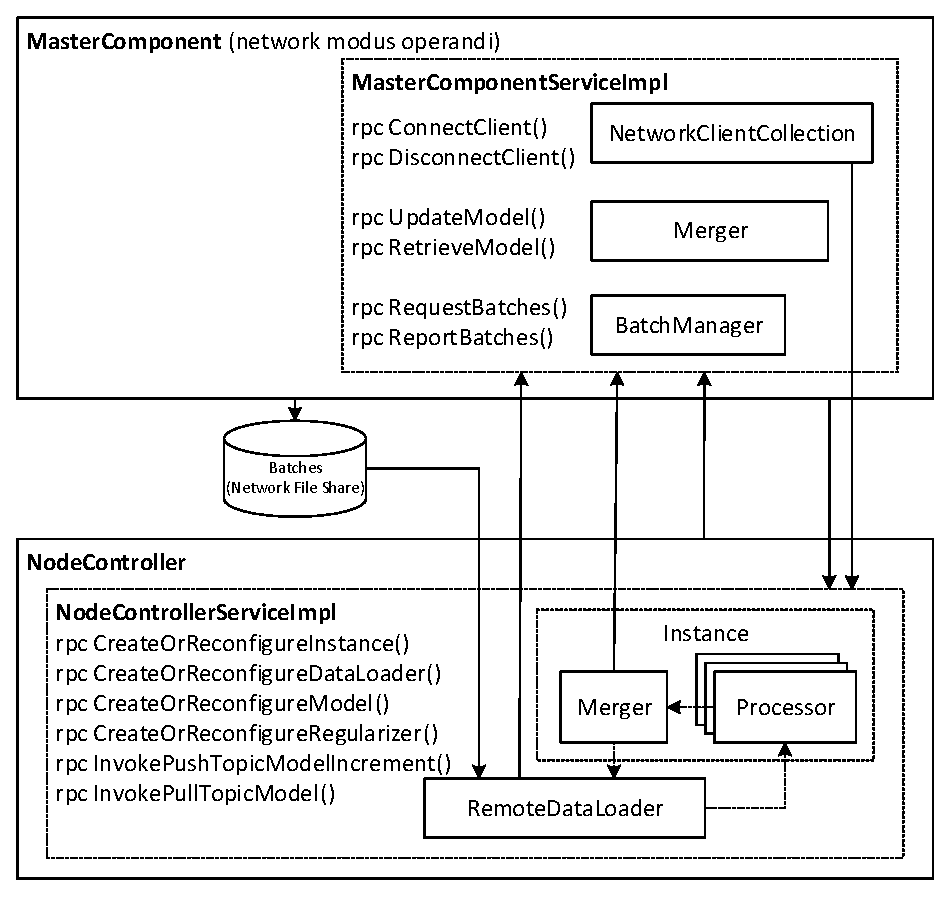
\includegraphics[height=84mm]{diagramm_artm_network.eps}
\caption{Diagram of ARTM components in network modus operandi}
\label{fig:diagramm_artm_network}
\end{centering}
\end{figure}
\vspace{1ex}

Interaction between MasterComponent and NodeControllers is implemented on \emph{RPCZ} technology.
Please, familiarize yourself with the concept of a
\href{en.wikipedia.org/wiki/Remote_procedure_call}{remote procedure call},
and read an overview of the following two libraries:
\href{code.google.com/p/rpcz/}{rpcz} and \href{http://zeromq.org}{ZeroMQ}.

\subsection{API in C++, Python and Java}
Currently the core ARTM functionality is only available from C++,
but it is designed to support Python and Java.

\begin{figure}[h!]
\begin{centering}
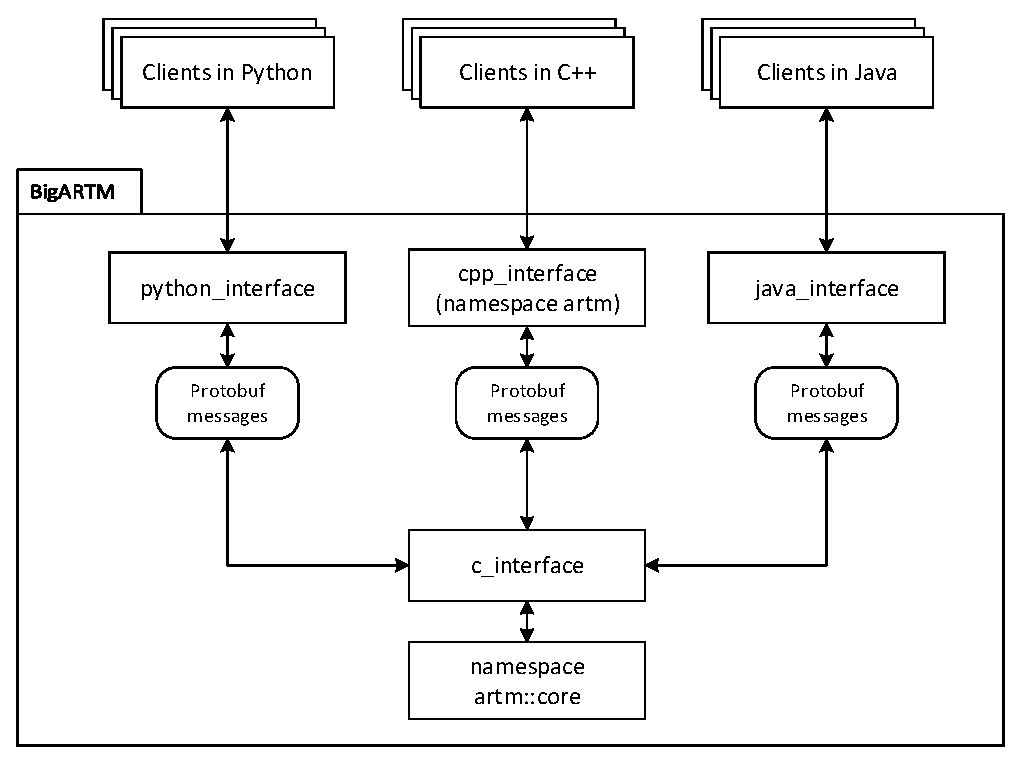
\includegraphics[width=90mm]{diagramm_BigARTM.eps}
\caption{Various interfaces on top of core ARTM components.}
\label{fig:diagramm_BigARTM}
\end{centering}
\end{figure}

\subsection{Concurrency and thread safety}
All interfaces of the library are not thread safe,
and must not be used concurrently from multiple threads.

Internally the library creates multiple threads
(one thread for each DataLoader, Processor and Merger).
Interaction between those threads is synchronized with the following locks:
\begin{enumerate}
    \item Lock access to the processors queue
    \item Lock access to the merger queue
    \item Lock access to the token-topic matrix
\end{enumerate}

We assume that batches are large enough,
and time to transfer a reference from dataloader to processor
is negligible comparing to processing time of one batch.
Access to token-topic matrix is read-only from processor,
so the lock is only needed to retrieve std::shared\_ptr.

DataLoader and Instance components also have their configuration objects,
which can be changed by user of the library during ongoing processing.
For those objects thread-safety is achieved by combining immutable pattern with std::shared\_ptr.
Look at /src/artm/core/thread\_safe\_holder.h for details.

\subsection{Data layout}
\begin{enumerate}
    \item Doc-token matrix: each doc is represented as list of token ids and their counts
    \item Token-topic matrix: each token is represented the list of topics and their probabilities
    \item Doc-topic matrix: each doc is represented as a sequential vector of topics (no sparsity)
\end{enumerate}

Due to caching in CPU it is important to have topics as a minor dimension in both token-topic and doc-topic matrices.

\subsection{Exceptions and error handling}

\textbf{In c\_interface} all error handling is happening through the error codes.
\begin{verbatim}
  enum ArtmErrorCodes {
    ARTM_SUCCESS = 0,
    ARTM_GENERAL_ERROR = -1,
    ARTM_OBJECT_NOT_FOUND = -2,
    ARTM_INVALID_MESSAGE = -3,
    ARTM_INVALID_OPERATION = -4,
  };
\end{verbatim}
You are free to add more error types when needed.
The reason for negative values is due to some API methods
returning the actual result; for example, this method returns an ID of newly created object.
\begin{verbatim}
int ArtmCreateDataLoader(int data_loader_id, int length,
                         const char* config);
\end{verbatim}

\textbf{In artm::core} you should use C++ exceptions
or simple true/false return values instead of error codes.
Please, follow guidelines in /artm/core/exceptions.h.
Some highlights:
\begin{enumerate}
    \item All exceptions should be inherited for std::runtime\_error
    \item Use BOOST\_THROW\_EXCEPTION macro to throw an exception
    \item Remember to catch all exceptions in c\_interface, and convert them to error codes.
\end{enumerate}

\textbf{In cpp\_interface} all error codes should be converted to exceptions.
Here you should use exceptions, defined in artm/core/cpp\_interface.h file.
Do not re-use existing exceptions from artm::core namespace.

\section{FAQ}

\subsection{What is ``google protocol buffers''}

For an overall introduction about google protocol buffers read the tutorial: \\
\url{https://developers.google.com/protocol-buffers/docs/cpptutorial} \\
Now take a look at file /src/artm/messages.proto,
and the compiled version (other messages.* files).

/src/artm/messages.proto describes the key objects that users can pass into our library.
For example, it defines the following entities:
\begin{itemize}
    \item the representation of a collection of textual files,
    \item all configuration parameters (number of concurrent processors, algorithm to use, etc),
    \item the representation of a topic model which library returns back to the user.
 \end{itemize}

For example, collection is represented as a set of Items.
Items is what you normally call ``documents'' --- they have a list of tokens (aka terms),
together with the number of occurrences of those tokens.
All tokens in each Item are organized into Field (for example, ``body'', ``author'', ``title'', ``year'').
This is a nice way of incorporating metadata into the document.

When passing items into the library those items should be organized into Batches.
Each batch is a collection of items, that share common dictionary of tokens.
Then each items is represented as two vectors --- indexes of tokens in the dictionary,
and the corresponding occurrences.

\paragraph{Key benefits of google protofol buffers}

Once you define you objects in .proto file, you can use them in many programming languages.
Google officially supports C++, Python, and Java. There are also good implementation for $\Csharp$.
I've also heard that it might be something for matlab, but I'm not so sure. Here is how it works:

1. Each proto-message has a serializer, which converts the message into byte array
(and corresponding deserializer that restores an original message).
The clue is that object can be serialized in one language (for example, in Python),
and deserialized in another language (for example, in C++).

2. Passing byte arrays between different languages is very simple.
If you have a .dll (or .so library in Linux) with "extern c" api,
you may call methods in this library from other languages.

As a result, the complex logic of the library can be written once in C++,
and then wrapped into many APIs, as in Fig. \ref{fig:diagramm_BigARTM}.

\subsection{There is so much code.. Where should I start?!}

First, take a look at /src/cpp\_client/srcmain.cc.
It is an example of a simple external application build on top of our library ---
it loads a collection of texts from a file,
splits this collections into batches, and sends them into the library.
Then the library tunes a model,
returns it back cpp\_client,
and the client reports top N words in each topic.

Try to run cpp\_client step by step in debugger and see what exactly it does.
To do so you have to unpack all archives under the /datasets folder,
and run cpp\_client with corresponding parameters.
In Linux you may simply use ``make kos'' or ``make nips'' commands.
To run cpp\_client in Windows directly from Visual Studio
you should configure the following command for debugger:

{\small
\begin{verbatim}
$(SolutionDir)..\datasets\docword.kos.txt $(SolutionDir)..\datasets\vocab.kos.txt 16
\end{verbatim}}

\section{Algorithms}

\subsection{Online PLSA}
Online PLSA is the only method implemented at the moment.
It has the following implementation details:
\begin{enumerate}
    \item Processing of documents happens in parallel, according to the design
    \item Strategy of updating matrix $\Phi$: after every scan of the whole collection.
          A next $\Phi$ matrix is accumulated from '0'.
          No exponential decay is currently implemented.
    \item Matrix Phi is initialized with random [0..1] values.
    \item By default distributions $\theta_{t d}$ are inferred from scratch on every scan of the collection.
          Processors can be configured to re-use the $\Theta$ values from previous iteration.
    \item Current perplexity calculation accumulates on test collection for every iteration.
    \item When p(w|d)=0 perplexity score uses unigram document model.
    \item Perplexity can be evaluated on testing items.
          Each item from the testing set is used to both infer theta, and evaluate perplexity.
          An alternative is to randomly split each testing document into two halves.
\end{enumerate}

\section{How to build sources?}
\label{label:how_to_build}

\subsection{C++ code on Windows}

\begin{enumerate}
   \item Download and install GitHub Windows from \url{http://windows.github.com/}
   \item Clone \url{https://github.com/sashafrey/topicmod/} repository
   \item Download and unpack boost 1.55  \\
         \url{http://sourceforge.net/projects/boost/files/} \\
         Set environmental variable BOOST\_ROOT to the root of your boost installation.
         To do so you may use cmd.exe:
\begin{verbatim}
setx BOOST_ROOT "C:\\Program Files\\boost\\boost_1_55_0"
\end{verbatim}
   \item \st{Download and unpack protobuf 2.5.0} \\ (no longer needed, part of '3rdparty' folder)
   \item Download and unpack the following libs into \verb'<topicmod>/libs' folder: \\
    \url{https://s3-eu-west-1.amazonaws.com/artm/libs_win32_v110.7z}
    Beware that this libraries were built with Visual Studio 2012 RTM (11.0.50727.1 RTMREL),
    and that they might be incompatible with future Service Packs for VS2012.
    They are known to be incompatible with Visual Studio 2013.
   \item Download and install \href{http://zeromq.org/distro:microsoft-windows}{ZeroMQ 4.0.3 x86} \\
         \url{http://miru.hk/archive/ZeroMQ-4.0.3~miru1.0-x86.exe} \\
         Set environmental variable ZEROMQ32\_ROOT to ZeroMQ include folder
\begin{verbatim}
setx ZEROMQ32_ROOT "C:\\Program Files (x86)\\ZeroMQ 4.0.3"
\end{verbatim}
    \item Install Visual Studio 2012 (other visual studio versions are not supported). \\
    \item Open /src/artm\_vs2012.sln
    \item Build all projects (debug or release, Win32) and execute tests. 64-bit builds are not available yet.
\end{enumerate}

\subsection{Python code on Windows}

\begin{enumerate}
	\item Install Python 2.7.

    {\bf Important:} on Windows you MUST use
    \href{https://www.python.org/ftp/python/2.7.6/python-2.7.6.msi}{Python x86},
    which is a 32bit version of Python. The 64bit Python is incompatible with artm.dll
    (which only compiles in 32 bits for now).

	\item Download and add to MSVS Python Tools 2.0.

    All necessary instructions can be found here:
	\url{https://pytools.codeplex.com/})
	\item Add python folder to PATH. To do so open:
\begin{verbatim}
    Control Panel\All Control Panel Items\System
\end{verbatim}
	then \verb'Advanced system settings', \verb'Environment variables'.
	\item Follow the instructions in README file in directory \verb'python'
    in your protobuf folder.
    In brief, this instructions ask you to run the following commands:
\begin{verbatim}
        python setup.py build
        python setup.py test
        python setup.py install
\end{verbatim}
    \verb'setup.py' is located under \verb'<topicmod>\3rdparty\protobuf\python'.
On second step you fill see two failing tests:
\begin{verbatim}
    Ran 216 tests in 1.252s
    FAILED (failures=2)
\end{verbatim}
    This 2 failures are OK to ignore.
\end{enumerate}

\subsection{Linux}

\begin{enumerate}
    \item Install git.
    \item git clone https://github.com/sashafrey/topicmod
    \item Install boost (it is preferable to use version 1.55 or newer; \hbox{libboost-all-dev} is package name in Debian-based OS).
    \item Install protobuf (it is necessary to use version 2.5.0 or newer; \hbox{libprotobuf-dev} is package name in Debian-based OS). You can get it from ppa: \hbox{ppa:chris-lea/protobuf}
    \item Use Makefiles under /3rdparty, /src/artm/ and /src/cpp\_client/.
    \item Python interface hasn't been used from Linux yet. Please, contribute to this documentation if you found some solution to this.
\end{enumerate}

\section{How to submit my change to master branch?}
\label{label:how_to_submit}
Every new feature should be developed in a separate git branch.
Usually the integrator (currently \href{mailto:sashafrey@gmail.com}{sashafrey@gmail.com})
merges this feature branches into the master branch.
The key responsibility of the integrator is to ensure stability of the master branch:
\begin{itemize}
    \item No build failures on Windows and on Linux
    \item No new compiler warnings
    \item All unit test passes
    \item Perplexity in cpp\_client looks reasonable
    \item Documentation is updated and compiles in LaTeX
    \item The change passed code review
    \item The change follows our code style
\end{itemize}
Everyone should periodically ``git pull master'' and merge master branch
into their feature branches.

In case if you are absolutely sure you change is safe, feel free to submit the change yourself.
Technically you do have write permissions, so no one can stop you :).
But please do the following:
verify your \hyperref[label:code_style]{code style},
perform \hyperref[label:code_review]{code review},
and make sure everything builds in both Linux and Windows, and unit test passes.

\subsection{Code style}
\label{label:code_style}
In the code we follow
\href{http://google-styleguide.googlecode.com/svn/trunk/cppguide.xml}{google code style},
with the following changes:
\begin{enumerate}
    \item Exceptions are allowed
    \item Indentation must be 2 spaces. Tabs are not allowed.

      If you use Visual Studio,
      please open ``Tools / Text Editor / All languages / Tabs''
      and configure as follows:
      \begin{itemize}
          \item Indenting "--- smart,
          \item Tab size "--- 2,
          \item Indent size "--- 2,
          \item Select "insert spaces".
      \end{itemize}

      We also suggest to show space and tab crlf characters (shortcut: Ctrl+R, Ctrl+W).
      \url{http://stackoverflow.com/questions/4065815/how-to-turn-off-showing-whitespace-characters-in-visual-studio-ide}

\item No lines should exceed 100 characters.

      If you use Visual Studio, please \href{http://stackoverflow.com/questions/9894397/100-characters-line-marker-in-visual-studio}{enable
       vertical line at 100 characters}.

\item All .h and .cpp files under /src/artm/ must be verified for code style with
      \href{http://google-styleguide.googlecode.com/svn/trunk/cpplint/cpplint.py}{cpplint.py} script.
      It is very easy to use the script; just install
      \href{http://www.python.org/downloads/}{Python 2.7.6}, and run

\begin{verbatim}
python cpplint.py --linelength=100 <filename>
\end{verbatim}
      Files, generated by protobuf compiler, are the only exceptions from this rule.

\end{enumerate}

\subsection{Code review}
\label{label:code_review}
We use
\href{https://code.google.com/p/rietveld/wiki/UploadPyUsage}{rietveld}
tool for code review.
When you have your first change, please learn how to use the
\href{http://codereview.appspot.com/static/upload.py}{unload.py} script.
For example, to upload all changes in between two git revisions you may use this command:
\begin{verbatim}
code review:
python upload.py --server=http://codereview.appspot.com/
 --email=<your_email> -t <review_title> -m <review_description>
 --rev=<from_revision>:<to_revision>
\end{verbatim}
where ``from\_revision'' and ``to\_revision'' may look as follows:
\begin{verbatim}
e26b8107520e219cac89f3cb6ed83b5680240a79
\end{verbatim}

\subsection{Language -- english or russian?}
Feel free to use either English or Russin in all e-mail conversations, including \url{https://groups.google.com/forum/#!forum/artm_dev}.

In the code everything should be in English only, including comments.
It is also preferable to keep this documentation in English.

\end{document}  